\titleformat{\subsection}
{\Large\bfseries\scshape\raggedright}
{\thesubsection}{1em}
{}
\titleformat{\subsubsection}
{\Large\bfseries\scshape\raggedright}
{\thesubsubsection}{1em}
{}
\titlespacing*{\section}{0pt}{*4}{*2}
\titlespacing*{\subsection}{0pt}{*4}{*2}
\titlespacing*{\subsubsection}{0pt}{*0}{*0}

\chapter{Definição da estratégia de mobilização e participação social}
\section{Mobilização Social}
De acordo com a PNRS (BRASIL, 2010), o controle social deverá ser realizado de modo que seja possível à sociedade ter acesso à informação e participar da implementação e da avaliação de políticas públicas voltadas ao tema dos resíduos sólidos. Assim, todos os mecanismos, ações e procedimentos que viabilizem esses objetivos de participação pública poderão ser entendidos como estratégias de controle social. 

Para promoção da participação e do controle social, são necessárias estratégias de comunicação e divulgação, e estratégias de mobilização social (ROMANI; SEGALA, 2014). De acordo com o Ministério do Meio Ambiente (MMA) e o ICLEI-Brasil (2012), a mobilização social pode ser entendida como uma mudança não apenas comportamental, mas também de hábitos, a qual ocorre, principalmente, por meio do diálogo e de ações orientadoras e provocativas, por parte do poder público. 

As estratégias para a mobilização social podem ser materializadas de diversas formas, a depender do alcance que se pretende. Para elaboração do Plano Nacional de Resíduos Sólidos, de abrangência nacional, foram adotadas audiências públicas regionais, audiência pública nacional e diversas consultas via internet (ROMANI; SEGALA, 2014). Em outro exemplo, em escala local, o município de São José dos Campos adotou as seguintes estratégias de mobilização social (SÃO JOSÉ DOS CAMPOS, 2015):
\begin{enumerate}
	\item Conscientização em domicílio;
	\item Palestras em ambientes públicos, como escolas, igrejas, ONGs, empresas etc.;
	\item Reuniões com diversos segmentos sociais;
	\item Mutirões de conscientização ambiental;
	\item Programa Lixo-Tour.
\end{enumerate}

\section{Metodologia}

As estratégias de mobilização social para o Plano Municipal de Gestão Integrada de Resíduos Sólidos de Monteiro Lobato foram elaboradas de modo que fosse possível conclamar toda a comunidade lobatense à participação no processo de construção e implementação do PMGIRS. Procurou-se levar em consideração, além das principais práticas já adotadas em outros planos do mesmo tema, as principais estratégias já adotadas no município, em iniciativas anteriores de mobilização social dentro do tema de gestão de resíduos sólidos, bem como a opinião de moradores e autoridades municipais. Essas estratégias foram desenvolvidas em três etapas:
\begin{enumerate}
	\item Diagnóstico, diálogo inicial e percepção de como a comunidade pode participar da elaboração e implementação do PMGIRS;
	\item Identificação de estratégias de mobilização social adotadas anteriormente pelo município;
	\item Estratégias para mobilizar a comunidade durante a elaboração, implementação, fiscalização e revisão do PMGIRS.
\end{enumerate}

\section{Diagnóstico e diálogo inicial}
 De acordo com vereadores e secretários municipais de Monteiro Lobato, a população lobatense pode ser classificada conforme descrito a seguir: 
 
\subsection{Morador tradicional}

Muito religioso (em sua maioria, católicos e evangélicos) esse tipo de morador é conservador, às vezes reacionário, avesso a mudanças radicais, 
Habita as áreas centrais do município, possui maior poder de compra e de decisão, em sua grande parte são donos de empreendimentos e estabelecimentos na cidade, ocupam cargos importantes no município, como os de vereadores e conselheiros da prefeitura. Tem maior escolaridade que os demais moradores, com vivências em outras regiões e municípios maiores, de grandes centros culturais, tais como as capitais estaduais brasileiras e de outros países do mundo.

\subsection{Morador de áreas rurais}

Representa a maioria dos moradores do município com traços mais tímido, menos participativos. O acesso a esse tipo de morador é restrito a pessoas de sua confiança e deve ser feito com grande cuidado. Esse tipo de morador possui baixa ou nenhuma escolaridade e pouca vivência fora dos limites do município.

\subsection{Novo morador}

É imigrante de outro município brasileiro, em geral, maior do que Monteiro Lobato.  O novo morador busca a tranquilidade característica do município, além de desfrutar do ambiente natural e fugir de problemas socioambientais de grandes centros urbanos. Esse tipo de morador possui nível de escolaridade maior do que a média do município, podendo manifestar opiniões sobre assuntos relacionados ao contexto municipal de forma elaborada, argumentada e crítica. O novo morador simpatiza-se com a ideia de conservação do ambiente natural e tranquilo, estando disposto a manifestar-se ativamente para que assim o ambiente do município seja mantido.

\subsection{Morador jovem}

Moradores jovens tendem a acessar a internet e as redes sociais com mais frequência, sendo mais ativos virtual do que fisicamente. É uma parcela da população que pouco se interessa em participar ativamente em atividades para a melhoria da qualidade ambiental do município. O jovem de Monteiro Lobato possui baixo nível de escolaridade, sendo que a maioria não estuda nem trabalha. Esse tipo de morador possui pouco interesse em sair da cidade e dificilmente dialoga sobre questões que extrapolam os assuntos compartilhados em redes sociais das quais participa.

\section{Estratégias adotadas anteriormente pelo município}

Grande parte das estratégias de educação ambiental e mobilização social para o desenvolvimento de ações de cuidado com os resíduos sólidos do município foram desenvolvidas tendo como núcleo de ação as escolas de ensino básico. Muitas dessas ações tinham como referencial principal o atual Instituto Pandavas, com o qual a Prefeitura estabeleceu parcerias de ação social e cuidado com o meio ambiente. O Instituto Pandavas – Núcleo de Educação, Cultura e Ações Socioambientais, existe desde 2008 e se propõe a dar continuidade aos trabalhos de educação ambiental, cidadania, justiça social e conservação da qualidade ambiental do município, desenvolvidos anteriormente pelo Centro Pedagógico Casa dos Pandavas – CPCP (PANDAVAS, 2017).

Nas décadas de 1990 e 2000, havia, no Centro Pedagógico Casa dos Pandavas, uma ONG chamada GARP – Grupo Ambientalista Ribeirão dos Pássaros. Essa ONG desenvolvia atividades para envolver pais, alunos e professores em ações e movimentos voltados à educação ambiental relacionada aos resíduos sólidos. Foram feitos mutirões, em que foram coletados materiais recicláveis nas ruas da cidade, em terrenos baldios e outras áreas de descarte irregular, com auxílio de caminhões que transportavam os resíduos coletados. Os mutirões foram feitos predominantemente em bairros da zona urbana; e em alguns locais da zona rural, como no Sousa e no São Benedito. Além disso, a ONG organizou a entrega de materiais escritos, nas áreas urbanas da cidade, de porta em porta, entre 1998 e 2000, com o objetivo de promover a educação ambiental e uma cultura de cuidado com os resíduos sólidos, visando a separação dos materiais em secos e úmidos. Na época, havia tratamento diferenciado para materiais recicláveis, os quais ficavam armazenados e eram triados em um galpão mantido pela Prefeitura.

Atualmente, não há continuidade de movimentos de educação ambiental envolvendo a comunidade lobatense da maneira como existia na época do CPCP; no entanto, trabalhos de cultura cinematográfica vêm sendo desenvolvidos, envolvendo jovens e adolescentes na discussão de temas importantes para o município. A Prefeitura participa ativamente na elaboração de vídeos e na escolha dos temas a serem abordados. 

\section{Estratégias propostas}

Levando em consideração as principais características do morador lobatense, além dos métodos já adotados no município com êxito para obtenção de participação da sociedade em projetos, foram elaboradas estratégias de participação e mobilização social, por meio das quais será possível convidar, envolver e esclarecer a comunidade sobre assuntos pertinentes à elaboração, implementação, fiscalização e revisão do PMGIRS. Todas as estratégias apresentadas a seguir foram validadas e elaboradas em consonância com a opinião dos secretários de meio ambiente e de educação, prefeita e vereadores, além de assessores técnicos atuantes na Prefeitura. Na \autoref{fig:danielepub} é possível visualizar o registro do dia em que ocorreu a entrevista com vereadores, a secretária de meio ambiente e técnicos assessores do serviço público municipal.

\begin{figure}
	\centering
	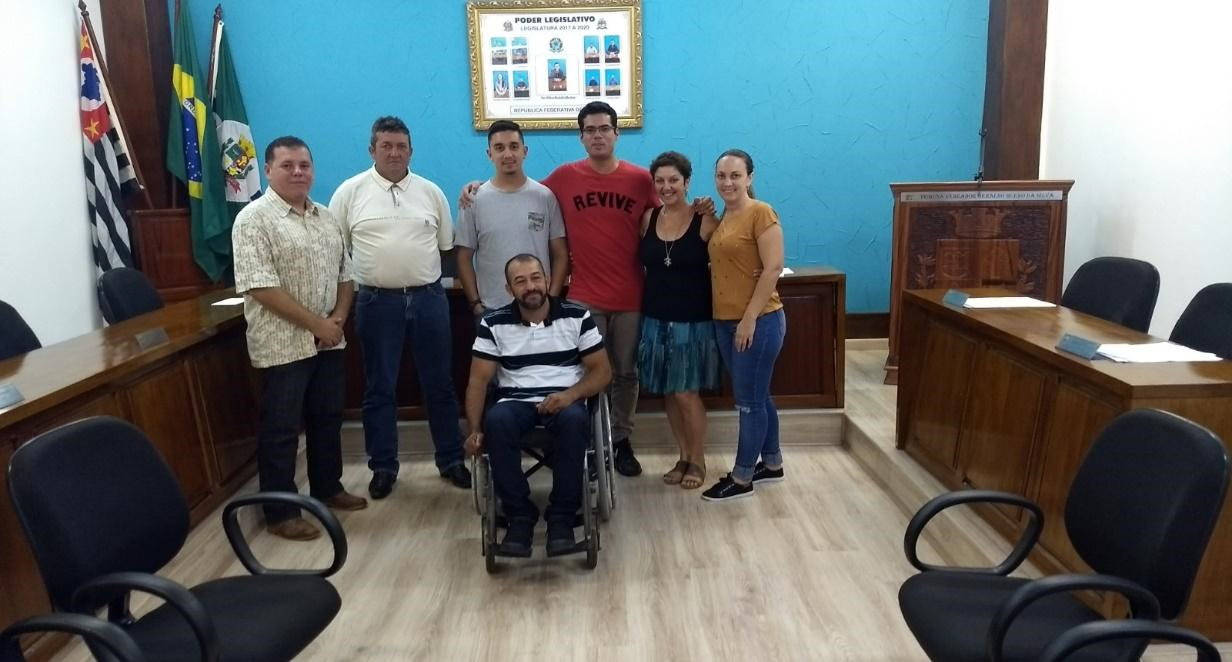
\includegraphics[width=\linewidth]{produtos/produm/danielepub}
	\caption{Encontro do estagiário Daniel com vereadores de Monteiro Lobato e integrantes da secretaria de meio ambiente}
	\label{fig:danielepub}
\end{figure}

O conteúdo das mensagens a serem distribuídas aos moradores, com o intuito de mobilização social, poderão abranger aspectos relacionados à logística dos resíduos (para coleta e para a destinação final), localização e tipo de material a ser usado em novas lixeiras, redução de geração de resíduos, custos do sistema de gestão e possibilidade de redução de custos em função da redução da geração dos resíduos, segurança no manuseio de resíduos, valorização do profissional que atua em contato direto com os resíduos, além da importância de separação dos tipos de resíduos gerados, na fonte geradora, entre inúmeros outros possíveis. Uma vez estabelecido o canal de comunicação com cada morador, poderão ser agendadas audiências públicas, reuniões entre líderes comunitários e representantes políticos, palestras, bem como festivais e eventos culturais para congregação de todos os interessados ou qualquer outra forma de comunicação e diálogo que convier no momento em que ocorrer a necessidade de diálogo e disseminação de informação entre comunidade e equipe responsável pela elaboração e implementação do PMGIRS.

No entanto, ressalta-se que o conteúdo específico a ser divulgado em cada etapa (elaboração, implementação, fiscalização e revisão) deverá ser definido em conjunto com todos os envolvidos e responsáveis pela elaboração do PMGIRS, o que inclui técnicos e servidores municipais. Nesta seção, será enfatizada a forma com que cada tipo de morador de Monteiro Lobato deverá ser abordado. Nesse contexto, as mensagens mobilizadoras deverão ser transmitidas com o intuito de provocar, orientar, mas também incitar o diálogo com a comunidade lobatense (MMA; ICLEI-BRASIL, 2012).

\subsection{Morador tradicional}

Deverá ser mobilizado de duas maneiras:
\begin{itemize}
	\item contato direto e pessoal, de porta em porta;
	\item contato indireto, por meio de igrejas e parcerias com líderes religiosos do município.
\end{itemize}

Na \autoref{fig:estrategmobi}, são apresentadas as etapas a serem seguidas para que se alcance o máximo de participantes de hábitos tradicionais.

\begin{figure}[h!]
	\centering
	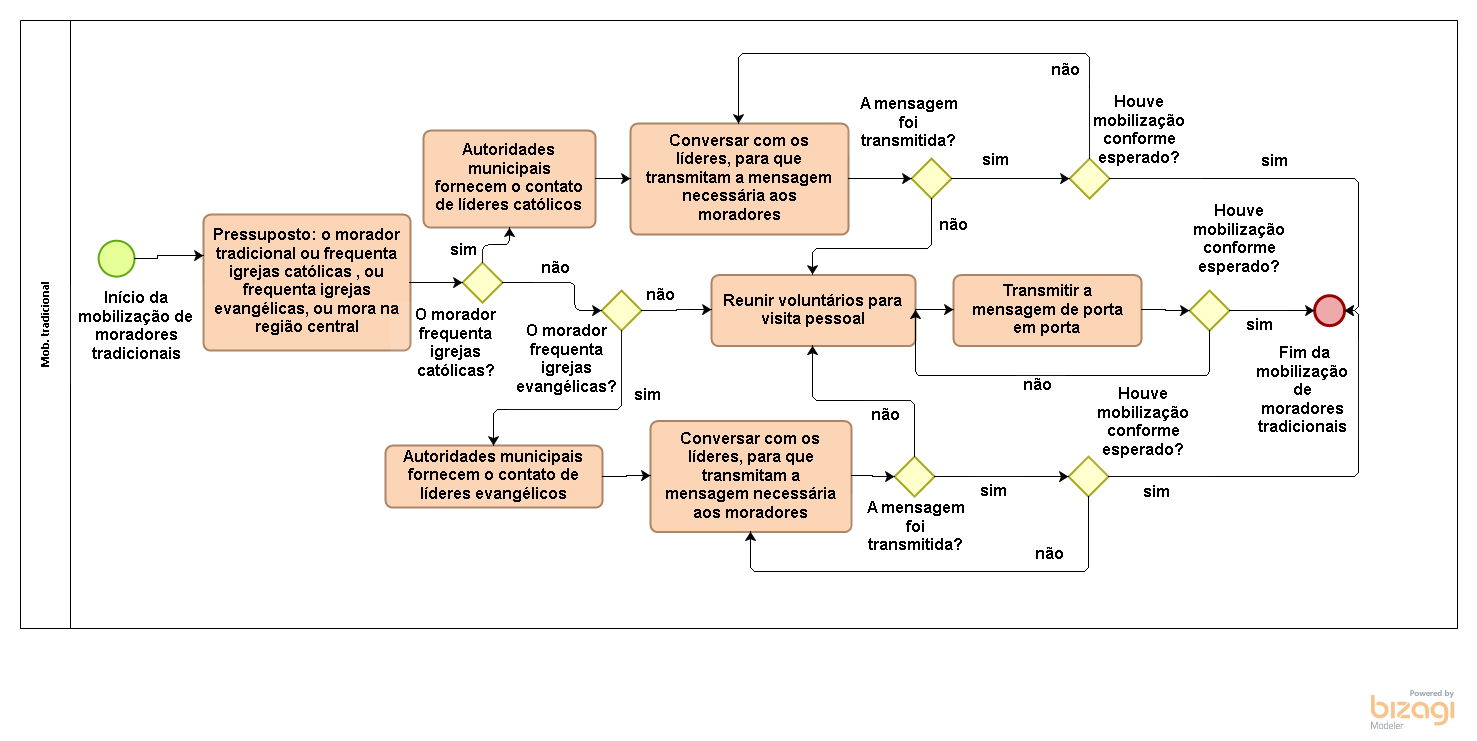
\includegraphics[width=\linewidth]{produtos/produm/estrategmobi}
	\caption{Estratégia de mobilização de moradores tradicionais}
	\label{fig:estrategmobi}
\end{figure}

Poderão ser reunidos como voluntários quaisquer alunos, servidores públicos ou munícipes devidamente treinados para conversar com o morador tradicional. No treinamento, deverão ser definidos:

\begin{itemize}
	\item Vestes a serem usadas;
	\item Linguagem e forma de abordagem;
	\item Conteúdo a ser transmitido;
	\item Tempo de fala;
	\item Conhecimento mínimo sobre o PMGIRS para que o visitante possa responder a eventuais
	perguntas dos moradores.
\end{itemize}

Em entrevista realizada na época de elaboração do plano, na câmara de vereadores de Monteiro Lobato, foi acordado entre vereadores e a secretária de meio ambiente, que os mesmos poderiam contribuir no acesso a líderes religiosos do município.

Deve-se também ressaltar a importância do estimulo fornecido pelo poder publico para que as associações de bairro realizem ações de mobilização mais efetiva da população.

\subsection{Morador de áreas rurais}

A mobilização da comunidade de áreas rurais será mais efetiva, caso as informações sobre a elaboração e implementação do PMGIRS sejam transmitidas por meio de pessoas de sua confiança, tendo como núcleo de ação as escolas rurais de ensino básico. Para que isso aconteça, apresenta-se na \autoref{fig:estrategmobiarearural} a estratégia por meio da qual será alcançada a participação comunitária, em etapas de execução na forma de um fluxograma.

\begin{figure}[h!]
	\centering
	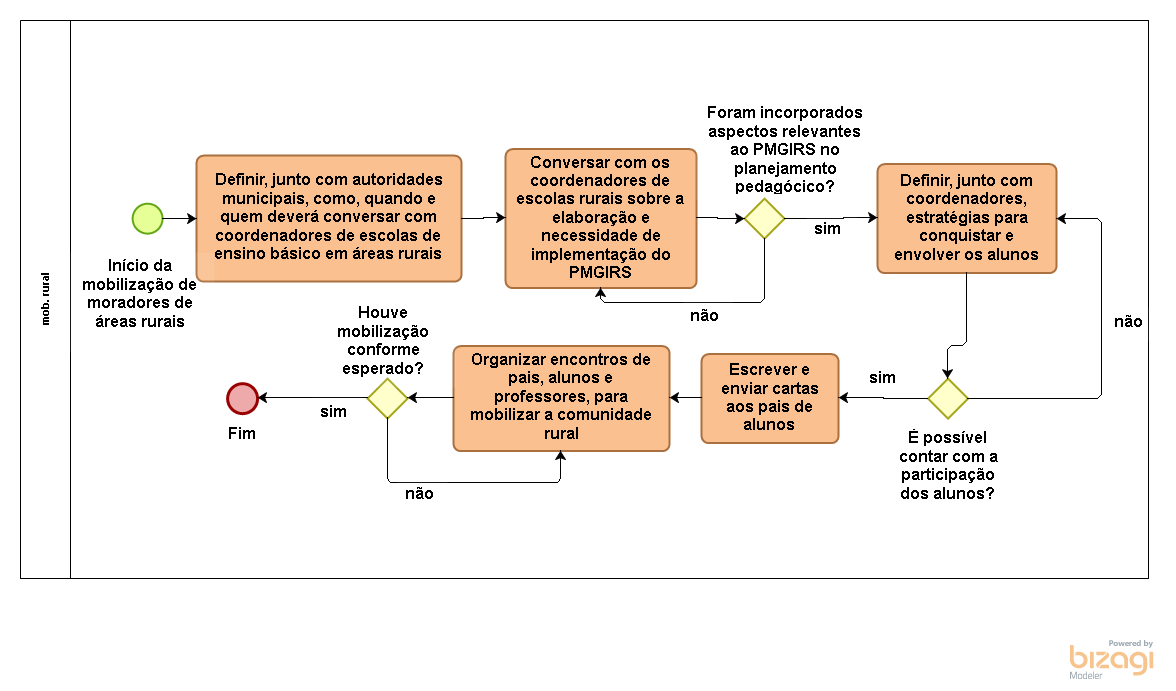
\includegraphics[width=\linewidth]{produtos/produm/estrategmobiarearural}
	\caption{Estratégia de mobilização de moradores de áreas rurais}
	\label{fig:estrategmobiarearural}
\end{figure}

A pessoa encarregada de conversar com os coordenadores de escolas rurais deverá saber se portar, comunicar, e transmitir de forma clara e precisa a necessidade de envolvimento das escolas na elaboração e implementação do PMGIRS. A tarefa poderá ser executada por um aluno estagiário ou não, com ou sem a apresentação de slides. Uma vez alcançado o comprometimento dos coordenadores de escolas e incorporada a temática de planejamento municipal da gestão dos resíduos sólidos no plano pedagógico de ensino, os alunos poderão ser envolvidos por meio de atividades diversas, tais como:
\begin{enumerate}
	\item Gincanas; 
	\item Redações; 
	\item Apresentações sobre o tema durante as aulas; 
	\item Estimulo de redução de consumo; 
	\item Visitas a locais de tratamento de resíduos, tais como um aterro sanitário ou uma cooperativa; 
	\item Mutirões para coleta de resíduos descartados irregularmente na área rural. 
\end{enumerate}

Com o apoio de coordenadores, educadores e alunos, os adultos, pais e familiares de áreas rurais, poderão ser envolvidos com maior facilidade, em encontros, reuniões, eventos escolares, etc. Assim, espera-se que um maior número da comunidade rural participará ou estará ciente de que sua participação é importante para o sucesso do PMGIRS.

\subsection{Turistas e visitantes}
A principal preocupação manifestada por autoridades municipais, em relação à visitação e turismo, refere-se ao respeito à dinâmica de separação dos tipos de resíduos e conservação da limpeza em todas as regiões visitadas, tanto no centro da cidade, como em pousadas mais afastadas do centro.  Além disso, foi ressaltada a importância de colaboração, por parte de todos os transeuntes (visitantes ou não), com as práticas e hábitos a serem implementados no município, em função das ações de implementação do PMGIRS. Assim, tendo como base essas preocupações principais, foi elaborada a estratégia para mobilização de visitantes e turistas, apresentada na \autoref{fig:estrategmobiturista}.

\begin{figure}[h!]
	\centering
	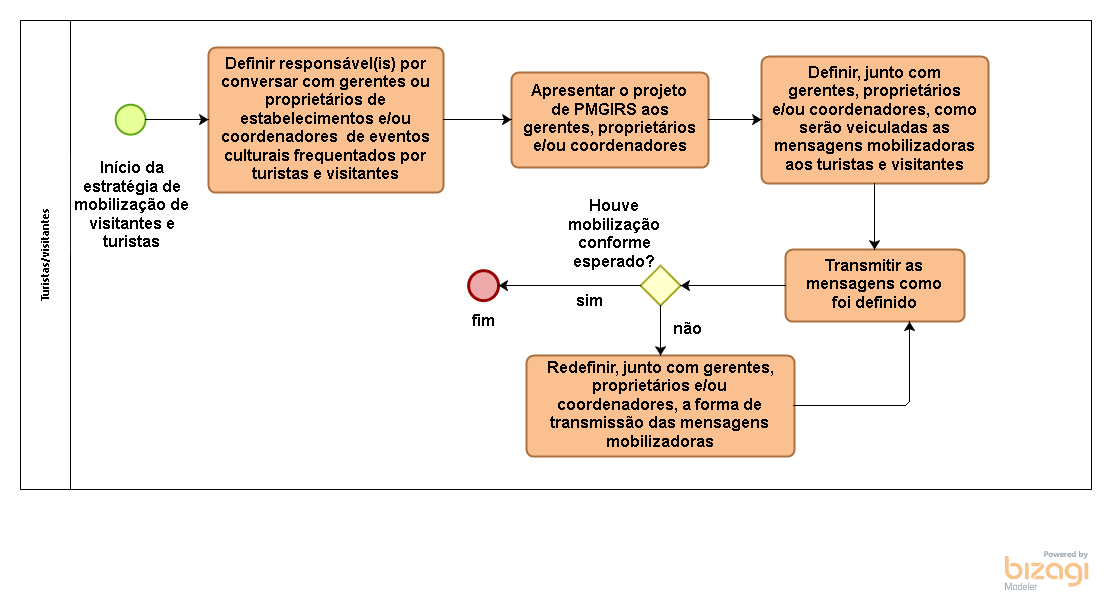
\includegraphics[width=\linewidth]{produtos/produm/estrategmobiturista}
	\caption{Estratégia de mobilização de visitantes e turistas}
	\label{fig:estrategmobiturista}
\end{figure}

Turistas e visitantes não são moradores; mas frequentam restaurantes, pousadas, hotéis e eventos culturais, gerando resíduos e podendo degradar a qualidade ambiental do município. Assim, deverão ser contatados a partir dos locais que frequentam, a partir de diálogo com donos de pousadas, hotéis, restaurantes e, eventualmente, coordenadores de festivais e eventos culturais em que haja aglomeração de pessoas, tais como o carnaval e festas de culinária e personagens de literatura infantil. A partir do diálogo com os gestores de estabelecimentos e locais turísticos, as ações de mobilização com foco nas necessidades de implementação ou elaboração do PMGIRS deverão ser elaboradas e executadas.


\subsection{Morador jovem}

Como jovem, entende-se o conjunto de moradores com idades entre 15 e 24 anos (IBGE, 2017).  Esse público, deverá ser contatado por meio de estratégias de encontros virtuais, conforme apresentado na \autoref{fig:estrategmobijovem}.

\begin{figure}[h!]
	\centering
	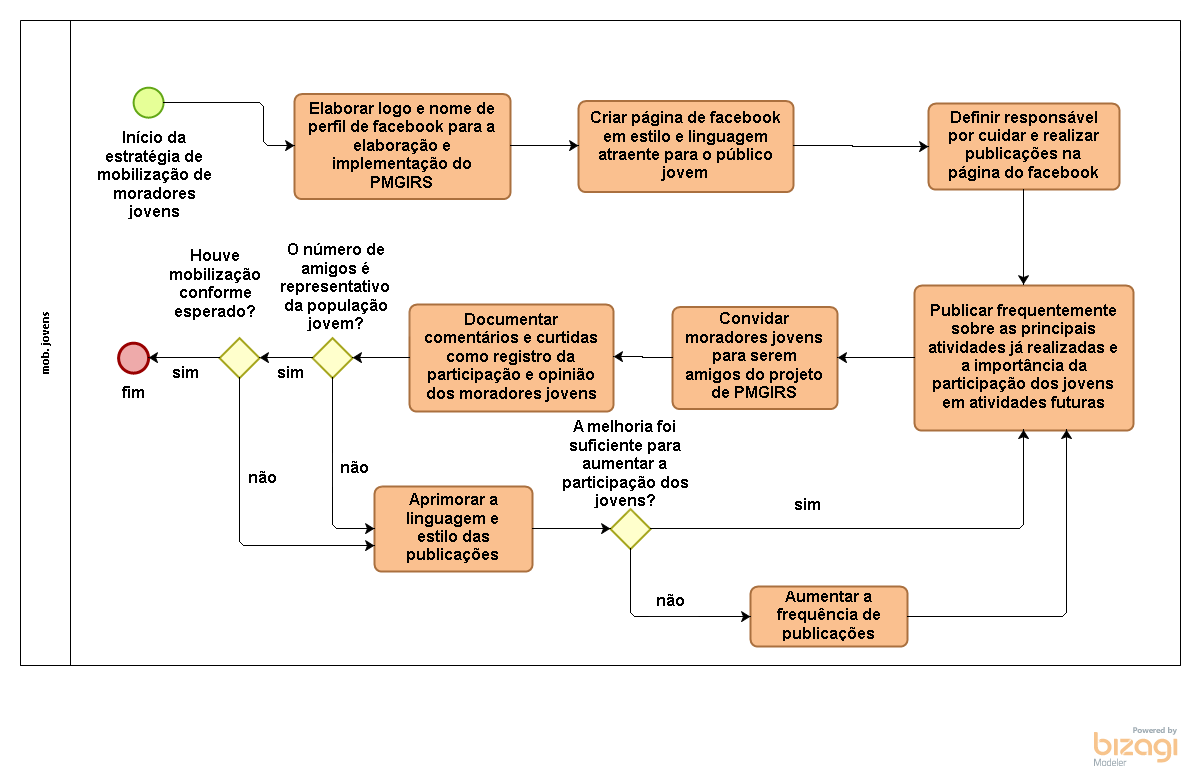
\includegraphics[width=\linewidth]{produtos/produm/estrategmobijovem}
	\caption{Estratégia de mobilização de moradores jovens}
	\label{fig:estrategmobijovem}
\end{figure}

O responsável por cuidar e realizar publicações na página criada do Facebook deverá ser definido em conjunto com autoridades do município e membros da equipe acadêmica responsável pela elaboração do PMGIRS. Sugere-se que a frequência de publicações seja diretamente proporcional à frequência com que novas ações sejam realizadas.

Para saber se o número de indivíduos com acesso à página é representativo ou não, sugere-se a adoção de uma proporção de representatividade a ser definida em conjunto com autoridades municipais. Essa proporção poderá ser, por exemplo, igual ou superior a 70\% da população de jovens do município (IBGE, 2017). Maiores informações sobre amostras significativas estão disponíveis em Bussab e Bolfarine (2005).


\section{Oficina para a apresentação do diagnóstico e discussões acerca da realização do prognóstico}

\subsection{Metodologia}

A oficina participativa é um instrumento amplamente utilizado para aproximar entidades públicas ou privadas de comunidades que são diretamente afetadas por ações, empreendimento ou políticas que possam alterar o cotidiano de uma população. Nessa prática, procura-se informar as condições dos locais que receberão tais ações, os estudos efetuados e resultados obtidos até o momento. A informação é passada de forma simples, direta e transparente cientificando e elucidando as informações à população, quanto ao andamento e às possíveis alterações que ocorrerão dentro de escopo apresentado.

A participação da população nessa etapa é de suma importância para o andamento das ações pretendidas, pois será neste momento que a população terá a possibilidade de fazer críticas/considerações sobre os dados apresentados e sobre as ações propostas, podendo também propor alternativas mais condizentes com as necessidades locais, bem como se informar sobre o andamento das ações.

Em Monteiro Lobato foram efetuadas 4 oficinas participativas (tabela q), de um total de 5 oficinas previstas, nas quais foi explicado aos participantes as condições relacionadas à produção, descarte, transporte e destinação dos resíduos sólidos do município. A estrutura da oficina é baseada em uma metodologia conhecida "Word Café". Esse sistema é um processo participativo com capacidade de trabalhar a diversidade e complexidade no grupo, fazendo emergir a inteligência coletiva. O processo é organizado de forma que as pessoas circulem entre os diversos grupos e conversas, conectando e semeando as ideias, tornando visível a inteligência e a sabedoria do coletivo. A oficina foi dividida em 3 etapas com 20 minutos cada: 

\begin{itemize}
	\item Apresentação dos dados municipais referentes aos resíduos gerados majoritariamente pela população (Resíduo Sólidos Urbano (RSU), Resíduos de Construção Civil (RCC), Resíduos de Serviços de Saúde (RSS) e logística reversa);
	\item Dinâmica inicial em grupo, por classe de resíduo ou conjunto de classes;
	\begin{itemize}
	\item Discussão interna feita pelos participantes sobre problemas relacionados à(s) classe(s) e seus possíveis motivos;
	\item descrição escrita em papéis separados sobre problemas e motivos destes problemas percebidos pela população;
	\item apresentação para todos os participantes das considerações feitas em grupo, seguida de rodas de discussão dos conteúdos apresentados e aprimoramento das ideias.
	\end{itemize}
	\item Dinâmica final em grupo, por classe de resíduo ou conjunto de classe;
	\begin{itemize}
	\item discussão interna sobre possíveis soluções relacionados à(s) classe(s) e como proporcionar seu acontecimento;
	\item descrição escrita em papéis separados sobre possíveis soluções e métodos para sua execução;
	\item apresentação para todos participante das considerações feitas seguida de rodas de discussão dos conteúdos apresentados e aprimoramento das ideias.
	\end{itemize}
\end{itemize}

A formação de grupos será realizada de acordo com os grandes grupos de classificação de resíduo, sendo que deve haver no mínimo dois grupos ou no máximo quatro, a escolha deve ser realizada de acordo com o número de participantes da oficina. Os objetivos principais são: promover a interação em conjunto dos participantes para identificar os principais problemas do município relacionados ao tratamento dos resíduos sólidos no município de Monteiro Lobato. Além disso deve ocorrer uma discussão mais especifica sobre os problemas comuns relacionados aos resíduos a que foram atribuídos ao grupo, bem como as soluções viáveis para mitigar os problemas encontrados e a magnitude dos impactos negativos e positivos, dos problemas e das soluções respectivamente. A etapa final da oficina consiste na troca de informações entre os grupos com apresentação das ideias e uma discussão entre os participantes.

